% IEEE standard conference template; to be used with:
%   spconf.sty  - LaTeX style file, and
%   IEEEbib.bst - IEEE bibliography style file.
% --------------------------------------------------------------------------

\documentclass[letterpaper]{article}
\usepackage{spconf,amsmath,amssymb,graphicx}

% Example definitions.
% --------------------
% nice symbols for real and complex numbers
\newcommand{\R}[0]{\mathbb{R}}
\newcommand{\C}[0]{\mathbb{C}}

% bold paragraph titles
\newcommand{\mypar}[1]{{\bf #1.}}

% Title.
% ------
\title{Implementation of an optimized authenticated encryption scheme}
%
% Single address.
% ---------------
\name{Alessandro Giaconia, Lorenzo Paleari, Diana Khimey, Filippo Visconti}
\address{Department of Computer Science\\ ETH Z\"urich\\Z\"urich, Switzerland}

% For example:
% ------------
%\address{School\\
%		 Department\\
%		 Address}
%
% Two addresses (uncomment and modify for two-address case).
% ----------------------------------------------------------
%\twoauthors
%  {A. Author-one, B. Author-two\sthanks{Thanks to XYZ agency for funding.}}
%		 {School A-B\\
%		 Department A-B\\
%		 Address A-B}
%  {C. Author-three, D. Author-four\sthanks{The fourth author performed the work
%		 while at ...}}
%		 {School C-D\\
%		 Department C-D\\
%		 Address C-D}
%

\begin{document}
%\ninept
%
\maketitle
%

% The hard page limit is 6 pages in this style. Do not reduce font size
% or use other tricks to squeeze. This pdf is formatted in the American letter format, so the spacing may look a bit strange when printed out.

\begin{abstract}
	% Describe in concise words what you do, why you do it (not necessarily
	% in this order), and the main result.  The abstract has to be
	% self-contained and readable for a person in the general area.
	You should write the abstract last.
\end{abstract}

\section{Introduction}\label{sec:intro}

% Do not start the introduction with the abstract or a slightly modified
% version. It follows a possible structure of the introduction.
% Note that the structure can be modified, but the
% content should be the same. Introduction and abstract should fill at most the first page, better less.

\mypar{Motivation}
% The first task is to motivate what you do.  You can
% start general and zoom in one the specific problem you consider.  In
% the process you should have explained to the reader: what you are doing,
% why you are doing, why it is important (order is usually reversed).
%
% For example, if my result is the fastest sorting implementation ever, one
% could roughly go as follows. First explain why sorting is important
% (used everywhere with a few examples) and why performance matters (large datasets,
% realtime). Then explain that fast implementations are very hard and
% expensive to get (memory hierarchy, vector, parallel).
%
% Now you state what you do in this paper. In our example:
% presenting a sorting implementation that is
% faster for some sizes as all the other ones.
In an era characterized by the exponential growth of data and the escalating prevalence of digital communication, safeguarding sensitive information has become an indispensable priority. The continuous evolution of technology introduces new challenges in upholding the confidentiality and integrity of data exchanged over networks.

This project embarks on a journey focused on implementing a state-of-the-art, optimized, high-performance authenticated encryption scheme. The motivation driving this initiative arises from the necessity for robust cryptographic solutions that not only ensure security but also exhibit efficient runtimes. Authenticated encryption schemes serve as fundamental pillars in modern cryptography, offering a comprehensive solution for ensuring the confidentiality, integrity, and authenticity of data. These schemes find widespread application in various contexts, including TLS, SSH, IPsec, and numerous others.

Our project leverages the combined strengths of ChaCha20 and Blake3, prioritizing efficiency and speed.

It's essential to note that the key distinction between authenticated encryption schemes and traditional encryption schemes lies in the former's ability to not only ensure confidentiality but also provide data integrity and authenticity, addressing the comprehensive security needs of modern applications.

\mypar{Related work} Next, you have to give a brief overview of
related work. For a report like this, anywhere between 2 and 8
references. Briefly explain what they do. In the end contrast to what
you do to make now precisely clear what your contribution is.

\section{Background}\label{sec:background}
In this section, we give a brief overview of the background necessary to understand the rest of the report.
In particular, we introduce the concepts of encryption and authentication, and we explain the algorithms we use.
% Give a short, self-contained summary of necessary
% background information. For example, assume you present an
% implementation of sorting algorithms. You could organize into sorting
% definition, algorithms considered, and asymptotic runtime statements. The goal of the
% background section is to make the paper self-contained for an audience
% as large as possible. As in every section
% you start with a very brief overview of the section. Here it could be as follows: In this section
% we formally define the sorting problem we consider and introduce the algorithms we use
% including a cost analysis.

\mypar{Encryption}
% Precisely define sorting problem you consider.

\mypar{Authentication}
Authentication is the process through which the integrity and origin of data are verified, to ensure that
t it remains untampered and confirming that it originated from the expected sender. This verification process holds significant importance in diverse fields, including secure communication, electronic commerce, and various other domains.

To achieve authentication, Message Authentication Code (MAC) is commonly employed. A MAC is a concise piece of information utilized to authenticate a message, working in conjunction with a secret key. The recipient of the message can validate its authenticity by recalculating the MAC and comparing it with the original MAC. This mechanism provides a secure means of ensuring that the received data has not been altered and originates from the expected source.

% As an aside, don't talk about "the complexity of the algorithm.'' It's incorrect,
% problems have a complexity, not algorithms.
\mypar{Blake3}
We opted for Blake3 as the authentication component of our scheme, driven by its notable combination of high performance and robust security guarantees. Blake3 is inherently parallelizable, enhancing its suitability for our implementation. The implementation, carried out in the C language, employs two distinct approaches: one utilizing a stack for versatility, and the other employing a more efficient divide-and-conquer strategy, albeit with slightly reduced flexibility, but significantly improved performance.

Blake3 operates as a cryptographic hash function with a built-in MAC function, the specific feature we are leveraging. At a high level, Blake3 processes input by dividing it into chunks of up to 1024 bytes and arranges them as the leaves of a binary tree. These chunks are then compressed using a compression function, conducting a series of operations on the input and producing a 64-byte output known as the chaining value. The chaining value from each chunk becomes the input for the subsequent chunk, and this process continues until all chunks are processed. The chunks effectively represent the leaves of a binary tree, and the tree is traversed from the bottom up. At each level, the chaining values of two children nodes are combined until reaching the root node. The final result is the chaining value of the root node, obtained through iterations of this process.

To obtain an output of arbitrary length, the last call to the compression function can be repeated with an increased counter, ensuring adaptability to various application requirements.

\section{Your Proposed Method}\label{sec:yourmethod}
In this section, we dive into the details of our implementation. We describe how we implemented the algorithms,
and we explain the optimizations we used to achieve high performance.
% Now comes the ``beef'' of the report, where you explain what you
% did. Again, organize it in paragraphs with titles. As in every section
% you start with a very brief overview of the section.
%
% In this section, structure is very important so one can follow the technical content.
%
\mypar{Blake3}
In this subsection, we describe our implementations of the Blake3 algorithm, which are based on and closely follow the original Blake3 paper that describes the algorithm in detail \cite{blake}.
Given their different strenghts and characteristics, we also included a dispatcher that chooses the best implementation based on the input size, to always guarantee a correct output.
\mypar{Stack version}
TODO

\mypar{Divide-and-conquer version}
The divide-and-conquer version of the algorithm relies on the premise that the entire input is accessible at the outset of the computation. This enables an equitable distribution of work among multiple threads, each operating on distinct portions of the input, and subsequently eliminating dependencies among them. The threads function concurrently until they reach the base case, wherein each thread is left with one node.

Upon reaching this base case, the threads transmit their individual results to the parent thread, which consolidates these outcomes and returns the final result. This parallelized approach enhances the algorithm's efficiency, leveraging the availability of the complete input early in the computation to facilitate concurrent and independent processing by multiple threads.
\begin{figure}[h]
	\begin{center}
		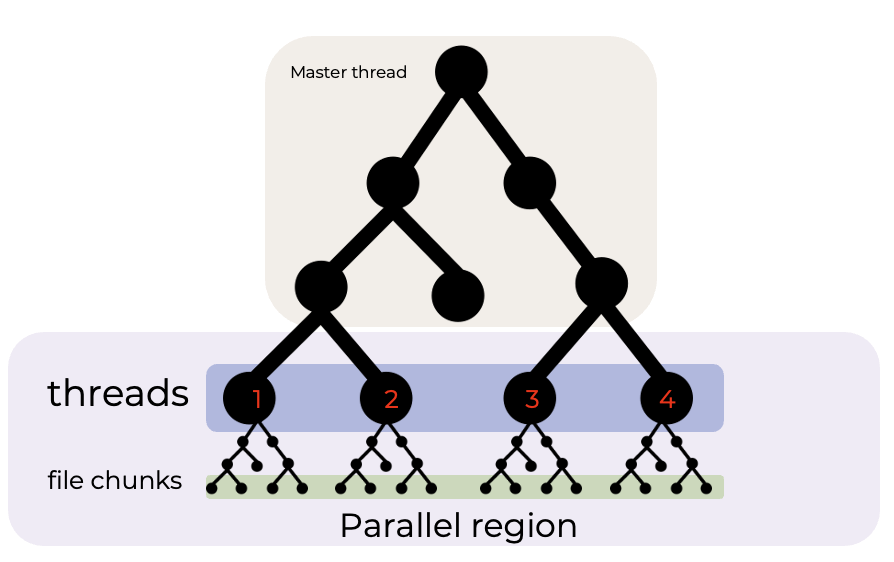
\includegraphics[width=0.45\textwidth]{figures/div_conq.png}
	\end{center}
	\caption{High-level visualization of the divide and conquer approach}\label{fig:divide_and_conquer}
\end{figure}

To facilitate parallelization in our algorithm, we leverage the OpenMP library, streamlining the process of distributing computation across threads once a parallel region is established. Additionally, we enhance performance by vectorizing the compression function, the most computationally intensive component of the algorithm, using the AVX instruction set and adopting code available on GitHub from the reference implementation.

The primary advantage of this approach lies in its scalability, attributed to the even distribution of work among threads with no inter-thread dependencies. This characteristic allows us to achieve commendable speedups, as detailed in the results section. However, it's important to note that this approach, while highly scalable, has limitations in flexibility. Specifically, it necessitates the availability of the entire input at the commencement of the computation (which aligns with our requirements) and is most effective when the input conforms to a full tree structure. These considerations, although relevant, are mitigated by the suitability of our use case.

TODO Mention and cite any external resources that you used including libraries or other code.

\section{Experimental Results}\label{sec:exp}

Here you evaluate your work using experiments. You start again with a
very short summary of the section. The typical structure follows.

\mypar{Experimental setup} Specify the platform (processor, frequency, maybe OS, maybe cache sizes)
as well as the compiler, version, and flags used. If your work is about performance,
I strongly recommend that you play with optimization flags and consider also icc for additional potential speedup.

Then explain what kind of benchmarks you ran. The idea is to give enough information so the experiments are reproducible by somebody else on his or her code.
For sorting you would talk about the input sizes. For a tool that performs NUMA optimization, you would specify the programs you ran.

\mypar{Results}
Next divide the experiments into classes, one paragraph for each. In each class of experiments you typically pursue one questions that then is answered by a suitable plot or plots. For example, first you may want to investigate the performance behavior with changing input size, then how your code compares to external benchmarks.

For some tips on benchmarking including how to create a decent viewgraph see pages 22--27 in \cite{Pueschel:10}.

{\bf Comments:}
\begin{itemize}
	\item Create very readable, attractive plots (do 1 column, not 2 column plots
	      for this report) with readable font size. However, the font size should also not be too large; typically it is smaller than the text font size.
	      An example is in Fig.~\ref{fftperf} (of course you can have a different style).
	\item Every plot answers a question. You state this question and extract the
	      answer from the plot in its discussion.
	\item Every plot should be referenced and discussed.
\end{itemize}

\begin{figure}\centering
	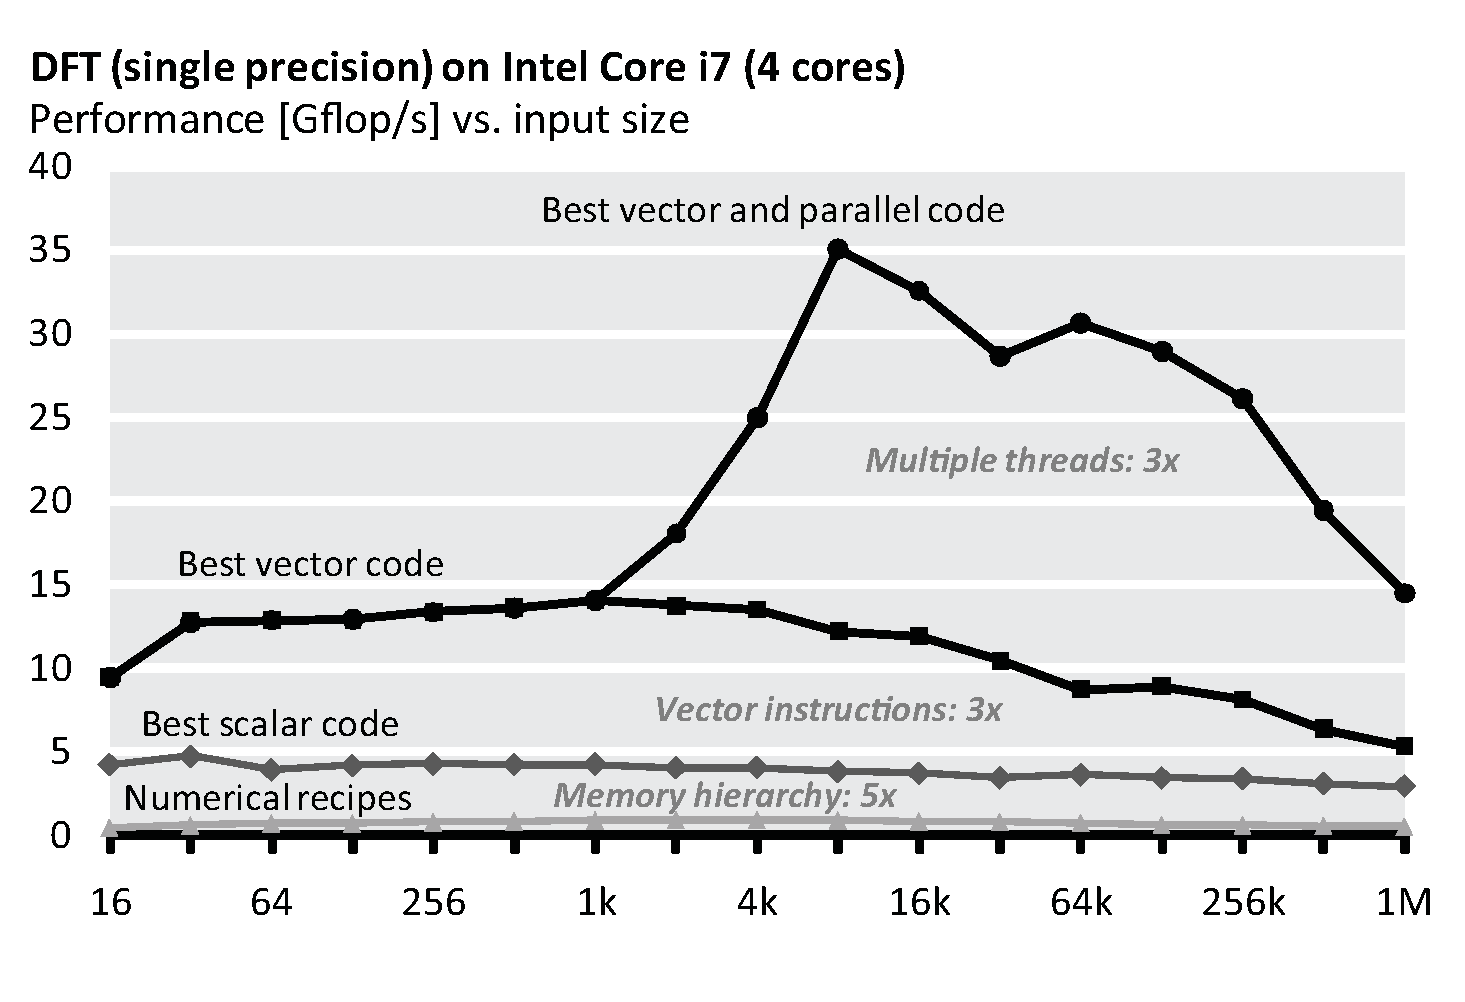
\includegraphics[scale=0.33]{dft-performance.eps}
	\caption{Performance of four single precision implementations of the
		discrete Fourier transform. The operations count is roughly the
		same. The labels in this plot are maybe a little bit too small.\label{fftperf}}
\end{figure}

\section{Conclusions}

Here you need to summarize what you did and why this is
important. {\em Do not take the abstract} and put it in the past
tense. Remember, now the reader has (hopefully) read the report, so it
is a very different situation from the abstract. Try to highlight
important results and say the things you really want to get across
such as high-level statements (e.g., we believe that .... is the right
approach to .... Even though we only considered x, the
.... technique should be applicable ....) You can also formulate next
steps if you want. Be brief. After the conclusions there are only the references.

\section{Further comments}

Here we provide some further tips.

\mypar{Further general guidelines}

\begin{itemize}
	\item For short papers, to save space, I use paragraph titles instead of
	      subsections, as shown in the introduction.

	\item It is generally a good idea to break sections into such smaller
	      units for readability and since it helps you to (visually) structure the story.

	\item The above section titles should be adapted to more precisely
	      reflect what you do.

	\item Each section should be started with a very
	      short summary of what the reader can expect in this section. Nothing
	      more awkward as when the story starts and one does not know what the
	      direction is or the goal.

	\item Make sure you define every acronym you use, no matter how
	      convinced you are the reader knows it.

	\item Always spell-check before you submit (to us in this case).

	\item Be picky. When writing a paper you should always strive for very
	      high quality. Many people may read it and the quality makes a big difference.
	      In this class, the quality is part of the grade.

	\item Books helping you to write better: \cite{Higham:98} and \cite{Strunk:00}.

	\item Conversion to pdf (latex users only):

	      dvips -o conference.ps -t letter -Ppdf -G0 conference.dvi

	      and then

	      ps2pdf conference.ps
\end{itemize}

\mypar{Graphics} For plots that are not images {\em never} generate the bitmap formats
jpeg, gif, bmp, tif. Use eps, which means encapsulate postscript. It is
scalable since it is a vector graphic description of your graph. E.g.,
from Matlab, you can export to eps.

The format pdf is also fine for plots (you need pdflatex then), but only if the plot was never before in the format
jpeg, gif, bmp, tif.


% References should be produced using the bibtex program from suitable
% BiBTeX files (here: bibl_conf). The IEEEbib.bst bibliography
% style file from IEEE produces unsorted bibliography list.
% -------------------------------------------------------------------------
\bibliographystyle{IEEEbib}
\bibliography{bibl_conf}

\end{document}
